\documentclass[12pt,a4paper]{article}
\usepackage[margin=1in]{geometry}
\usepackage[T1]{fontenc}
\usepackage[utf8]{inputenc}
\usepackage{lmodern}
\usepackage{setspace}
\usepackage{enumitem}
\usepackage{booktabs}
\usepackage{longtable}
\usepackage{array}
\usepackage{tabularx}
\usepackage{hyperref}
\usepackage{xcolor}
\usepackage{tikz}
\usetikzlibrary{arrows.meta,positioning,shapes.geometric}

\hypersetup{colorlinks=true,linkcolor=blue,urlcolor=blue,citecolor=blue}
\setstretch{1.12}
\setlength{\parskip}{0.45em}
\setlength{\parindent}{0pt}

\title{Project Report\\\large EEG Based Motor Imagery Classification}
\author{Team: [Add member names and roles]}
\date{09-Apr-2026}

\begin{document}
\maketitle

\section*{Abstract}
This project implements a Brain Computer Interface pipeline for EEG motor imagery classification. The system includes a Python backend and a web frontend with two screens: Screen A for EEG stream visualization and target class control, and Screen B for live prediction and confidence display. The model training pipeline uses GDF files with strict train and evaluation split logic and class-aware selection. Current baseline training uses four cue classes: left, right, foot, and tongue.

\section{Introduction}
Motor imagery classification is a core BCI task where imagined movements are decoded from EEG. This project focuses on building an end-to-end implementation suitable for lab demonstration and iterative research development.

\section{Literature Review Summary Plan}
The final review must include papers from 2023 to 2025 and complete all mandatory tables.

\subsection{Objectives Mapping Table (Mandatory)}
\begin{longtable}{p{0.12\textwidth}p{0.30\textwidth}p{0.10\textwidth}p{0.38\textwidth}}
\toprule
\textbf{Paper No.} & \textbf{Title} & \textbf{Year} & \textbf{Objectives Addressed} \\
\midrule
P1 & [Fill] & [Fill] & [Fill] \\
P2 & [Fill] & [Fill] & [Fill] \\
P3 & [Fill] & [Fill] & [Fill] \\
P4 & [Fill] & [Fill] & [Fill] \\
P5 & [Fill] & [Fill] & [Fill] \\
P6 & [Fill] & [Fill] & [Fill] \\
P7 & [Fill] & [Fill] & [Fill] \\
P8 & [Fill] & [Fill] & [Fill] \\
P9 & [Fill] & [Fill] & [Fill] \\
\bottomrule
\end{longtable}

\subsection{Datasets Used in Reviewed Papers (Mandatory)}
\begin{longtable}{p{0.10\textwidth}p{0.23\textwidth}p{0.30\textwidth}p{0.27\textwidth}}
\toprule
\textbf{Paper No.} & \textbf{Dataset Name} & \textbf{Dataset Link} & \textbf{Purpose} \\
\midrule
P1 & [Fill] & [Fill] & [Fill] \\
P2 & [Fill] & [Fill] & [Fill] \\
P3 & [Fill] & [Fill] & [Fill] \\
P4 & [Fill] & [Fill] & [Fill] \\
P5 & [Fill] & [Fill] & [Fill] \\
P6 & [Fill] & [Fill] & [Fill] \\
P7 & [Fill] & [Fill] & [Fill] \\
P8 & [Fill] & [Fill] & [Fill] \\
P9 & [Fill] & [Fill] & [Fill] \\
\bottomrule
\end{longtable}

\section{Objective of Our Project}
\begin{itemize}[leftmargin=1.5em]
  \item Build a real-time MI classification pipeline from EEG.
  \item Support four MI classes based on cue onset events:
  \begin{itemize}[leftmargin=1.5em]
    \item 769 left
    \item 770 right
    \item 771 foot
    \item 772 tongue
  \end{itemize}
  \item Provide a clear frontend for stream interaction and classifier interpretation.
\end{itemize}

\section{Experimental Dataset}
Dataset files available in project folder:
\begin{itemize}[leftmargin=1.5em]
  \item Four-class files:
  \begin{itemize}[leftmargin=1.5em]
    \item Training: A01T to A09T
    \item Evaluation: A01E to A09E
  \end{itemize}
  \item Two-class files:
  \begin{itemize}[leftmargin=1.5em]
    \item Training: B0101T to B0903T
    \item Evaluation: B0104E to B0905E
  \end{itemize}
\end{itemize}

Dataset links:
\begin{itemize}[leftmargin=1.5em]
  \item BCI Competition IV: \url{https://www.bbci.de/competition/iv/}
  \item BNCI Horizon: \url{http://bnci-horizon-2020.eu/database/data-sets}
\end{itemize}

Dataset protocol used in project:
\begin{itemize}[leftmargin=1.5em]
  \item Only T files are used for training.
  \item E files are reserved for evaluation.
  \item For strict four-class training, files must contain all four cues.
\end{itemize}

\section{Preprocessing Methods}
\begin{itemize}[leftmargin=1.5em]
  \item Channel selection and mapping to analysis layout
  \item Bandpass filtering: 0.5 to 40 Hz
  \item Notch filtering: 50 Hz
  \item Per-channel normalization
  \item Epoch extraction from cue-related segments
  \item Feature extraction from mu and beta band behavior
\end{itemize}

\section{ML/DL Approaches}
Current baseline:
\begin{itemize}[leftmargin=1.5em]
  \item MLP-based lightweight classifier integrated into checkpoint runtime.
\end{itemize}

Planned DL upgrades:
\begin{itemize}[leftmargin=1.5em]
  \item EEGNet baseline for EEG-specific spatial-temporal patterns
  \item CNN-LSTM for temporal context
  \item Transformer-lite for sequence modeling
\end{itemize}

\section{Proposed Block Diagram}
\begin{figure}[h!]
\centering
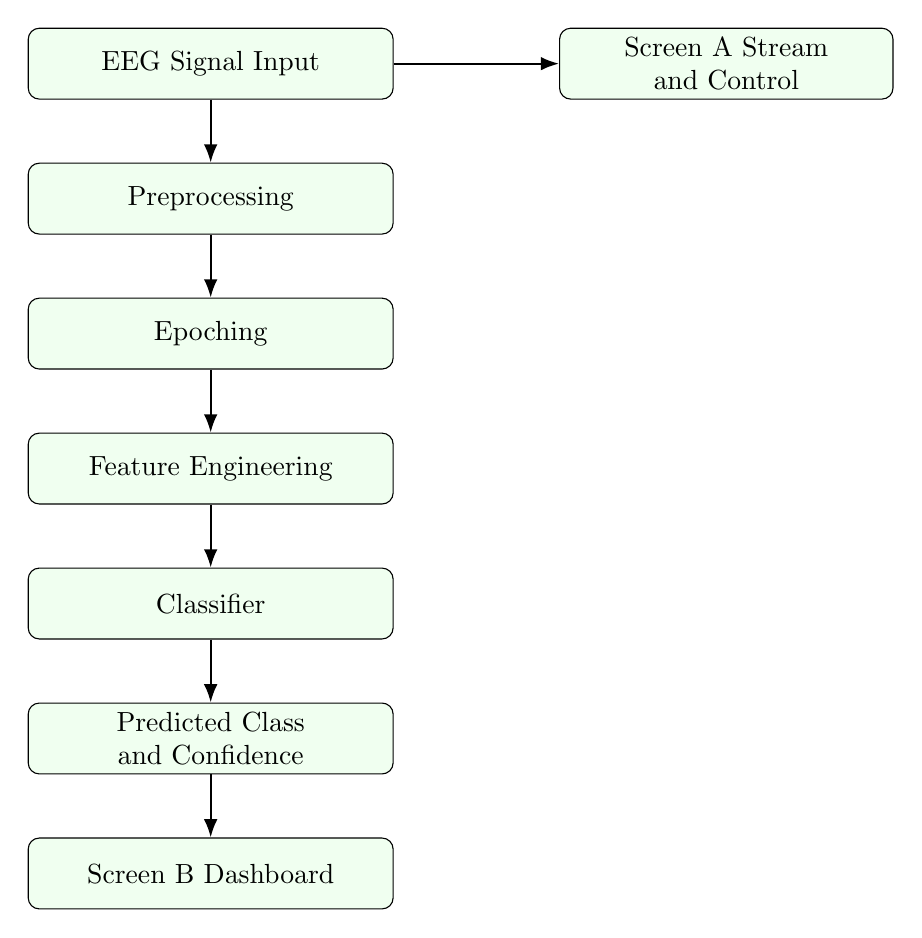
\begin{tikzpicture}[
  node distance=0.8cm,
  block/.style={rectangle, rounded corners, draw=black, align=center, minimum height=0.9cm, text width=4.4cm, fill=green!6},
  arrow/.style={-Latex, thick}
]
\node[block] (a) {EEG Signal Input};
\node[block, below=of a] (b) {Preprocessing};
\node[block, below=of b] (c) {Epoching};
\node[block, below=of c] (d) {Feature Engineering};
\node[block, below=of d] (e) {Classifier};
\node[block, below=of e] (f) {Predicted Class and Confidence};
\node[block, below=of f] (g) {Screen B Dashboard};
\node[block, right=2.1cm of a, text width=4.0cm] (h) {Screen A Stream\\and Control};

\draw[arrow] (a) -- (b);
\draw[arrow] (b) -- (c);
\draw[arrow] (c) -- (d);
\draw[arrow] (d) -- (e);
\draw[arrow] (e) -- (f);
\draw[arrow] (f) -- (g);
\draw[arrow] (a.east) -- (h.west);
\end{tikzpicture}
\caption{Project pipeline block diagram}
\end{figure}

\section{Implementation Tools and Libraries}
\begin{itemize}[leftmargin=1.5em]
  \item Backend: Python, FastAPI, Uvicorn
  \item Signal and ML stack: NumPy, SciPy, MNE, scikit-learn
  \item Frontend: HTML, CSS, JavaScript, Canvas
  \item Documentation and diagrams: Markdown, draw.io
\end{itemize}

\section{Current Implementation Status}
Implemented:
\begin{itemize}[leftmargin=1.5em]
  \item Real-time synthetic EEG stream and controls
  \item WebSocket pipeline from backend to frontend
  \item Live prediction with confidence trend
  \item Retraining script from dataset GDF files
  \item Class-aware training file filter
\end{itemize}

\section{Baseline Training Results (Current)}
Latest strict four-class retraining summary:
\begin{itemize}[leftmargin=1.5em]
  \item Files used: A01T to A09T
  \item Class counts:
  \begin{itemize}[leftmargin=1.5em]
    \item \texttt{left\_hand}: 648
    \item \texttt{right\_hand}: 648
    \item \texttt{feet}: 648
    \item \texttt{tongue}: 648
  \end{itemize}
  \item Hold-out test accuracy: about 26.6\%
\end{itemize}

Interpretation:
\begin{itemize}[leftmargin=1.5em]
  \item Pipeline correctness is validated.
  \item Baseline model quality is limited for four-class MI and needs improved model/feature design.
\end{itemize}

\section{Challenges and Observations}
\begin{itemize}[leftmargin=1.5em]
  \item Strong inter-subject variability in EEG patterns.
  \item Domain mismatch between synthetic stream and real recorded data can affect live behavior.
  \item Four-class discrimination is harder than two-class left-right setup.
\end{itemize}

\section{Improvement Plan}
\begin{itemize}[leftmargin=1.5em]
  \item Add CSP/FBCSP-based features.
  \item Add EEGNet training and compare with baseline.
  \item Add kappa score and per-subject evaluation.
  \item Add robust calibration layer for live inference.
\end{itemize}

\section{Project Timeline (Date-to-Date)}
\begin{longtable}{p{0.44\textwidth}p{0.16\textwidth}p{0.16\textwidth}p{0.14\textwidth}}
\toprule
\textbf{Task} & \textbf{Start Date} & \textbf{End Date} & \textbf{Duration} \\
\midrule
SRS report and PPT preparation & 10-Apr-2026 & 12-Apr-2026 & 3 days \\
Data preprocessing & 13-Apr-2026 & 15-Apr-2026 & 3 days \\
ML/DL baseline implementation & 16-Apr-2026 & 18-Apr-2026 & 3 days \\
Final model and hyperparameter tuning & 19-Apr-2026 & 22-Apr-2026 & 4 days \\
Result analysis and comparison & 23-Apr-2026 & 25-Apr-2026 & 3 days \\
\bottomrule
\end{longtable}

\section{Conclusion}
The project currently provides a complete end-to-end BCI workflow from EEG input simulation to online classification display. Data split and cue-class training rules are correctly enforced. The next stage is to improve model performance for robust four-class motor imagery decoding.

\section{References (To Finalize)}
\begin{itemize}[leftmargin=1.5em]
  \item Add all selected papers from 2023 to 2025 in IEEE format.
  \item Add dataset references and tool documentation links.
\end{itemize}

\end{document}
